\documentclass{article}

% Language setting
\usepackage[english]{babel}

% Set page size and margins
\usepackage[letterpaper,top=2cm,bottom=2cm,left=3cm,right=3cm,marginparwidth=1.75cm]{geometry}

% Useful packages
\usepackage{amsmath}
\usepackage{graphicx}
\usepackage[colorlinks=true, allcolors=blue]{hyperref}
\usepackage{float}
\DeclareMathOperator*{\argminA}{arg\,min}

\title{CS461 HW 3}
\author{John Bailon}
\date{November 17, 2024}

\begin{document}
\maketitle

\section{Decision Trees}
\subsection{Information Gained}

First, we will define entropy and conditional entropy. Entropy is a measure of uncertainty or randomness in a random variable and is given by the following formula

\[H(Y) = - \sum_{i}{P(Y = y_i)\log_2{P(Y =y_i)}}\]

where $P(Y=y_i)$ is the probability of each target class value.

Conditional entropy represents that amount of uncertainty in Y given X and is given by the following formula

\[H(Y|X) = \sum_{j}{P(X = x_j)H(Y | X = x_j)} = \sum_{i}{P(X = x_i) \sum_{i}{P(Y = y_i | X = x_j)\log_2{P(Y = y_i | X = x_j)}}}\]

Finally, mutual information is the difference between these two values and represents the information gained by knowing the value of feature X. To construct the tree, we will calculate the mutual information for each feature and split the data based on the feature with the greatest mutual information. 

For brevity, the full calculations of the first feature is shown. Afterwards, only the probabilities are shown.
\[P(Y = Yes) = P(Y = No) =  \frac{5}{10} = 0.5\]
\[H(Y) = - ((0.5 * \log_2(0.5)) + (0.5 * \log_2(0.5))) = 1\]

Weather:
\[P(X = Sunny) = \frac{3}{10} = 0.3\]
\[P(X = Cloudy) = \frac{3}{10} = 0.3 \]
\[P(X = Rainy) = \frac{4}{10} = 0.4 \]

\[P(Y= True | X = Sunny) =  \frac{1}{3} = 0.33 \]
\[P(Y= True | X = Cloudy) = \frac{3}{3} = 1 \]
\[P(Y= True | X = Rainy) = \frac{1}{4} = 0.25 \]

\[P(Y = False | X = Sunny) = 1 - 0.33 = 0.67\]
\[P(Y = False | X = Cloudy) = 1 - 1 = 0  \]
\[P(Y = False | X = Rainy) = 1- 0.25 = 0.75 \]

\[H(Y|Weather) = (0.3*-(0.33*\log_2{0.33} + 0.67*\log_2{0.67})) + 0.3*-\log_2{1} + (0.4*-(0.25*\log_2{0.25} + 0.75*\log_2{0.75})) = 0.6\]

\[I(Weather;Y) = 1 - 0.6 = 0.4\]

Temperature:
\[P(X = Hot) =  0.4\]
\[P(X = Mild) = 0.5 \]
\[P(X = Cool) = 0.1 \]

\[P(Y= True | X = Hot) = 0.5 \]
\[P(Y= True | X = Mild) = 0.6 \]
\[P(Y= True | X = Cool) = 0 \]

\[P(Y = False | X = Hot) = 0.5 \]
\[P(Y = False | X = Mild) = 0.4\]
\[P(Y = False | X = Cool) = 1\]

\[H(Y|Temperature) = 0.8855\]

\[I(Temperature;Y) = 1 - 0.8855 = 0.1145\]

Humidity:
\[P(X = High) =  0.7\]
\[P(X = Normal) = 0.3 \]

\[P(Y= True | X = High) = 0.43 \]
\[P(Y= True | X = Normal) = 0.67 \]

\[P(Y = False | X = High) = 0.57 \]
\[P(Y = False | X = Normal) = 0.33\]

\[H(Y|Humidity) = 0.9651\]

\[I(Humidity;Y) = 1 - 0.9651 = 0.0349\]

Wind:
\[P(X = Strong) =  0.6\]
\[P(X = Weak) = 0.4 \]

\[P(Y= True | X = Strong) = 0.33 \]
\[P(Y= True | X = Weak) = 0.75 \]

\[P(Y = False | X = Strong) = 0.67 \]
\[P(Y = False | X = Weak) = 0.25\]

\[H(Y|Wind) = 0.8755\]

\[I(Wind;Y) = 1 - 0.8755 = 0.1245\]

The feature with the greatest information is weather. Thus, we will split the data into three groups based on weather- Sunny, cloudy, rainy.

\subsection{Pure Tree}
After splitting the tree, the cloudy set has achieved purity and does not need to be split further.

Looking at sunny:
\[P(Y = Yes) = 0.333\]
\[PP(Y = No) = 0.667\]
\[H(Y) = 0.918\]

Temperature:
\[P(X = Hot) =  0.67\]
\[P(X = Mild) = 0.33 \]
\[P(X = Cool) = 0\]

\[P(Y= True | X = Hot) = 0 \]
\[P(Y= True | X = Mild) = 1 \]
\[P(Y= True | X = Cool) = 0 \]

\[P(Y = False | X = Hot) = 1 \]
\[P(Y = False | X = Mild) = 0\]
\[P(Y = False | X = Cool) = 0\]

\[H(Y|Temperature) = 0\]

\[I(Temperature;Y) = 0.918 - 0 = 0.918\]

Humidity:
\[P(X = High) =  0.67\]
\[P(X = Normal) = 0.33 \]

\[P(Y= True | X = High) = 0 \]
\[P(Y= True | X = Normal) = 1 \]

\[P(Y = False | X = High) = 1 \]
\[P(Y = False | X = Normal) = 0\]

\[H(Y|Humidity) = 0\]

\[I(Humidity;Y) = 0.918 - 0 = 0.918\]

Wind:
\[P(X = Strong) =  0.67\]
\[P(X = Weak) = 0.33 \]

\[P(Y= True | X = Strong) = 0.50 \]
\[P(Y= True | X = Weak) = 0 \]

\[P(Y = False | X = Strong) = 0.5 \]
\[P(Y = False | X = Weak) = 1\]

\[H(Y|Wind) = 0.667\]

\[I(Wind;Y) = 0.918 - 0.667 = 0.251\]

Here, both temperature and humidity give the same information. I will split by high and low humidity, leading to two pure leaf nodes.

Finally, let's look at Rainy
\[P(Y = Yes) = 0.25\]
\[PP(Y = No) = 0.75\]
\[H(Y) = 0.811\]

Temperature:
\[P(X = Hot) =  0\]
\[P(X = Mild) = 0.75 \]
\[P(X = Cool) = 0.25\]

\[P(Y= True | X = Hot) = 0 \]
\[P(Y= True | X = Mild) = 0.33 \]
\[P(Y= True | X = Cool) = 0 \]

\[P(Y = False | X = Hot) = 0 \]
\[P(Y = False | X = Mild) = 0.67\]
\[P(Y = False | X = Cool) = 1\]

\[H(Y|Temperature) = 0.6887\]

\[I(Temperature;Y) = 0.811 - 0.6887 = 0.1226\]

Humidity:
\[P(X = High) =  0.75\]
\[P(X = Normal) = 0.25 \]

\[P(Y= True | X = High) = 0.33 \]
\[P(Y= True | X = Normal) = 0 \]

\[P(Y = False | X = High) = 0.67 \]
\[P(Y = False | X = Normal) = 1\]

\[H(Y|Humidity) = 0.6887\]

\[I(Humidity;Y) = 0.811 - 0.6887 = 0.1226\]

Wind:
\[P(X = Strong) =  0.75\]
\[P(X = Weak) = 0.25 \]

\[P(Y= True | X = Strong) = 0 \]
\[P(Y= True | X = Weak) = 1 \]

\[P(Y = False | X = Strong) = 1 \]
\[P(Y = False | X = Weak) = 0\]

\[H(Y|Wind) = 0\]

\[I(Wind;Y) = 0.811 - 0 = 0.811\]

Here, wind gives the most information. Splitting wind by strong and weak, we have two pure leaf nodes as well.

The final tree is shown below.

\begin{figure}[H]
    \centering
    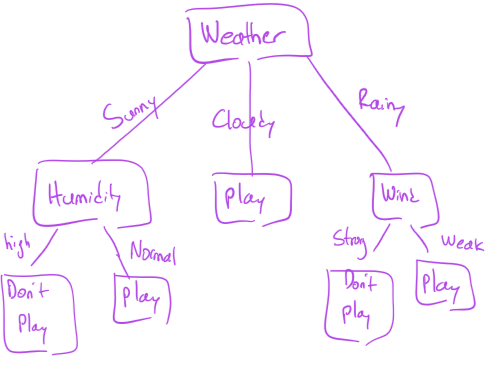
\includegraphics[width=0.5\linewidth]{1.2 Tree.png}
    \caption{Completed 1.2 Decision Tree}
\end{figure}


\subsection{Pruning Trees}

To prune trees we want to minimize the following criterion

\[C(T') = \sum_{\tau = 1}^{T'} Q(\tau) + \lambda * | num Leaves in T' |\]

\[Q(\tau) = H(\tau) = - \sum P(\tau)\log_{2}{P(\tau)}\]

Of note, a pure leaf has an entropy of 0. So in the current tree, the criterion of the unpruned tree is

\[C(T') =  5\lambda\]

We will start by looking at nodes that we can prune. We can select either weather, humidity, or wind to prune. The criterion of the tree can be calculated by looking at the entropy of the resulting leaf node post-prune. 

Wind
\[P(Y = Yes) = 0.25\]
\[ P(Y = No) = 0.75\]
\[H(Y) = - ((0.25 * \log_2(0.25)) + (0.75 * \log_2(0.75))) = 0.8113\]

\[C(T') = 0.8113 + 4\lambda \]

Humidity
\[P(Y = Yes) = 0.33\]
\[P(Y = No) = 0.67\]
\[H(Y) = - ((0.33 * \log_2(0.33)) + (0.67 * \log_2(0.67))) = 0.9183\]

\[C(T') = 0.9183 + 4\lambda \]

Weather
\[P(Y = Yes) = P(Y = No) = 0.5\]
\[C(T') =  1 + \lambda\]

From here we can evaluate various lambdas to see which criterion is minimized. 

\[\lambda = 0 \]
\[C(T') =  5(0) = 0\]
\[C(T') = 0.8113 + 4(0) = 0.8113 \]
\[C(T') = 0.9183 + 4(0) = 0.9183\]
\[C(T') =  1 + (0) = 1\]

\[\lambda = 0.25 \]
\[C(T') =  5(0.25) = 1.25\]
\[C(T') = 0.8113 + 4(0.25) = 1.8113 \]
\[C(T') = 0.9183 + 4(0.25) = 1.9183\]
\[C(T') =  1 + (0.25) = 1.25\]

\[\lambda = 1 \]
\[C(T') =  5(1) = 5\]
\[C(T') = 0.8113 + 4(1) = 4.8113 \]
\[C(T') = 0.9183 + 4(1) = 4.9183\]
\[C(T') =  1 + (1) = 2\]

Here we see that from 0 to 0.25, the criterion is minimized without pruning. For values greater than 0.25, it is optimal to prune the whole tree. Given that the data set is small (n=10) a lower value is optimal such as 0.1. The tree that minimizes this is the original tree, so nothing should be pruned.


\section{Perceptron}
\subsection{Iterations- Single Data Point}
With an initial $w_0$ = (0,0) and step size of 1, let's look at the initial prediction of the data point $\{(x_1, x_2), +1\}$

\[y_{pred} = w_1x_1 + w_2x_2\]
\[y_{pred} = (0)x_1 + (0)x_2 = 0 \rightarrow -1\] 

This is an incorrect prediction so we will update weights by the following rule.

\[w = w + \eta(y_{true})(x_1)\]

\[w_1 = 0 + (1)(1)(x_1) = x_1\]
\[w_2 = 0 + (1)(1)(x_2) = x_2\]

Next, let's look at the second prediction.

\[y_{pred} = (x_1)x_1 + (x_2)x_2 = x_1^2 + x_2^2\]

As long as the point is not centered at the origin, the above sum, is always positive. This results in a correct prediction. Therefore, for all points except $(x_1, x_2) = (0,0)$ Perceptron will find a decision boundary in 1 iteration.

\subsection{Iterations- Random weight vector}
Let's look at two cases. If the initialized weights result in a correct prediction, then no updates are required. 

If there is a misclassification, then we need to update the weights. The generalized rule for weight updates for n updates is

\[w_1* = w_1 + nx_1 \]
\[w_2* = w_2 + nx_1\]

Then the nth prediction will be
\[y_{pred} = (w_1 + nx_1)x_1 + (w_2 + nx_2)x_2\]
\[y_{pred} = w_1x_1 + nx_1^2 + w_2x_2 + nx_2^2\]
\[y_{pred} = w_1x_1 + w_2x_2 + n(x_1^2 + x_2^2)\]

To get the correct classification, 

\[w_1x_1 + w_2x_2 + n(x_1^2 + x_2^2) > 0\]

Solving for n, the number of iterations before correct classification is
\[n = \left \lceil{\frac{-(w_1x_1 + w_2x_2)}{(x_1^2 + x_2^2)}}\right \rceil \]

\subsection{Perceptron Walk-through}

Iteration 2- Mismatch, Point 3
\[1: (0)(0) + (1)(1) = 1 \rightarrow +1\]
\[2: (0)(1) + (1)(1) = 1 \rightarrow +1\]
\[3: (0)(1) + (1)(0.5) = 0.5 \rightarrow +1\]

\[w_2 = (0,1) + (-1)(1, 0.5) = (-1,0.5)\]

Iteration 3- Mismatch, Point 2
\[1: (-1)(0) + (0.5)(1) = 0.5 \rightarrow +1\]
\[2: (-1)(1) + (0.5)(1) = -0.5 \rightarrow -1\]
\[3: (-1)(1) + (0.5)(0.5) = -0.75 \rightarrow -1\]

\[w_3 = (-1,0.5) + (1)(1, 1) = (0, 1.5)\]

Iteration 4- Mismatch, Point 3
\[1: (0)(0) + (1.5)(1) = 1.5 \rightarrow +1\]
\[2: (0)(1) + (1.5)(1) = 1.5 \rightarrow +1\]
\[3: (0)(1) + (1.5)(0.5) = 0.75 \rightarrow +1\]

\[w_4 = (0, 1.5) + (-1)(1, 0.5) = (-1,1)\]

Iteration 5- Mismatch, Point 2
\[1: (-1)(0) + (1)(1) = 1 \rightarrow +1\]
\[2: (-1)(1) + (1)(1) = 0 \rightarrow -1\]
\[3: (-1)(1) + (1)(0.5) = -0.5 \rightarrow -1\]

\[w_5 = (-1,1) + (1)(1, 1) = (0,2)\]

Iteration 6 Mismatch, Point 3
\[1: (0)(0) + (2)(1) = 2 \rightarrow +1\]
\[2: (0)(1) + (2)(1) = 2 \rightarrow +1\]
\[3: (0)(1) + (2)(0.5) = 1 \rightarrow +1\]

\[w_6 = (0,2) + (-1)(1, 0.5) = (-1,1.5)\]

Iteration 7- Complete
\[1: (-1)(0) + (1.5)(1) = 1.5 \rightarrow +1\]
\[2: (-1)(1) + (1.5)(1) = 0.5 \rightarrow +1\]
\[3: (-1)(1) + (1.5)(0.5) = -0.25 \rightarrow -1\]

\section{Gaussian Discriminant Analysis}
\subsection{Data Statistics}

\[
\begin{array}{|c|c|c|}
\hline
Class & Mean & Var \\
\hline
Class + & -0.0722 & 1.3097 \\
\hline
Class - & 0.9401 & 1.9437 \\
\hline
\end{array}
\]

\subsection{Test Accuracy}
The test accuracy is 61.50\%.

\subsection{Classifier Improvements}
We can improve the decision rule by considering the priors of the data set. Considering priors minimizes the expected classification error. It also improves generalization and regulates over-fitting as it lowers the likelihood probability.

The test accuracy is 90.00\%.

\subsection{GDA- 2D Data Statistics}

Class+ 

Mean: (0.01307, 0.06295) 
Covariance:

\[
\begin{array}{|c|c|}
\hline
 0.98285498 & 0.006120467 \\
\hline
 0.00612046 & 1.05782804 \\
\hline
\end{array}
\]

Mean: (-0.02314, -0.02115) 
Covariance:

\[
\begin{array}{|c|c|}
\hline
 1.00329037 & -0.01142356 \\
\hline
 -0.01142356 & 4.97693356 \\
\hline
\end{array}
\]

\subsection{2D Test Accuracy}
The test accuracy is 84.00\%.

\subsection{Specified Densities}
The test accuracy is 85.00\%. This is a slight, but not a very significant increase in the GDA model found in 3.4. GDA is a reasonable framework for classification especially if the underlying data follows a normal distribution or is very close to it, as seen in 3.5. GSA also considers priors, which minimize expected classification errors.

\section{Logistic Regression}
\subsection{Data Reprocessing}
Term frequency-Inverse Document frequency describes how important a word is in relation to the document or corpus it is a part of. It is comprised of two parts: Term frequency and inverse document frequency.

Term frequency is the ratio of the number of times a given word is in a document and the number of words in the document.

Inverse document frequency is the log of the total number of documents over the number of documents that has a given word.

TF-IDF is the product of term frequency and inverse document frequency. It highlights important words that are not common across all documents.

\subsection{Dimensionality Reduction}
See attached code.

\subsection{Model Creation}
See attached code.

\subsection{Train and Test Accuracy}
The training accuracy is 96.37\% and the test accuracy is 96.20\%. 

\subsection{mail.txt Example}
To test, I added the mail.txt to the enron dataset, ran the preprocessing file, and data4.2 file. I extracted the mail and tested it against my model.

Probability 99.64\% that it is spam.


\end{document}